

\documentclass[11pt,letterpaper,oneside,openany,article]{memoir}

% =====================
% Memoir package config
% =====================
\counterwithout{section}{chapter}
\setsecnumdepth{subsection}
\setulmarginsandblock{1in}{1in}{*}
\setlrmarginsandblock{1in}{1in}{*}
\tightlists

\checkandfixthelayout
% =====================


\usepackage{graphicx}
\usepackage{authblk}
\usepackage{hyperref}
\usepackage{upquote}
\usepackage{verbatim}
\usepackage{url}
\usepackage{subcaption}
\usepackage{amsmath}
\usepackage{tabularx}
\usepackage{multirow}

\usepackage{scrextend}

\usepackage{enumitem}

\usepackage{listings}
\lstset{language=bash,
 % How/what to match
    sensitive=true,
    % Border
	frame=single,
    % Put extra space under caption
    belowcaptionskip=1\baselineskip,
    % Colors
    backgroundcolor=\color{sbase3},
    basicstyle=\small\color{sbase00}\ttfamily,
    keywordstyle=\color{scyan},
    commentstyle=\itshape\color{sbase1},
    stringstyle=\color{sblue},
    numberstyle=\scriptsize\color{sviolet},
    identifierstyle=\color{sbase00},
    % Break long lines into multiple lines?
    breaklines=true,
    tabsize=2
}

\usepackage[normalem]{ulem}  % provides strikeout with \sout{...}

\usepackage[T1]{fontenc}
\usepackage{newpxtext, newpxmath}
\usepackage[scaled=0.8]{beramono}

\newcommand{\code}[1]{\lstinline{#1}}
\usepackage{xcolor}

\def\marrow{{\marginpar[\hfill$\longrightarrow$]{$\longleftarrow$}}}

\def\kobus #1 {{\textcolor{red}{ \scshape \newline\newline Kobus says: }{\marrow\sffamily #1 \newline\newline}}}
\def\clay #1 {{\textcolor{blue}{ \scshape \newline\newline Clay says: }{\marrow\sffamily #1 \newline\newline}}}
\newcommand{\Adarsh}[1]{{\color{Maroon} \scshape Adarsh:} {\sffamily #1}}
\def\eduong #1 {{\textcolor{magenta}{ \scshape \newline\newline Eric D. says: }{\marrow\sffamily #1 \newline\newline}}}
\def\cjs #1 {{\textcolor{pink}{ \scshape \newline\newline Caleb says: }{\marrow\sffamily #1 \newline\newline}}}

% I am not sure what these do for us, and when. Maroon and RoyalBlue should be
% defined by package xcolor.
%
\definecolor{webgreen}{rgb}{0,.5,0}
\definecolor{webbrown}{rgb}{.6,0,0}
\definecolor{Maroon}{cmyk}{0, 0.87, 0.68, 0.32}
\definecolor{RoyalBlue}{cmyk}{1, 0.50, 0, 0}
\definecolor{Black}{cmyk}{0, 0, 0, 0}
\definecolor{shadecolor}{gray}{0.9}
\definecolor{sbase03}{HTML}{002B36}
\definecolor{sbase02}{HTML}{073642}
\definecolor{sbase01}{HTML}{586E75}
\definecolor{sbase00}{HTML}{657B83}
\definecolor{sbase0}{HTML}{839496}
\definecolor{sbase1}{HTML}{93A1A1}
\definecolor{sbase2}{HTML}{EEE8D5}
\definecolor{sbase3}{HTML}{FDF6E3}
\definecolor{syellow}{HTML}{B58900}
\definecolor{sorange}{HTML}{CB4B16}
\definecolor{sred}{HTML}{DC322F}
\definecolor{smagenta}{HTML}{D33682}
\definecolor{sviolet}{HTML}{6C71C4}
\definecolor{sblue}{HTML}{268BD2}
\definecolor{scyan}{HTML}{2AA198}
\definecolor{sgreen}{HTML}{859900}


\PassOptionsToPackage{dvipsnames}{xcolor}
    \RequirePackage{xcolor} % [dvipsnames]

\PassOptionsToPackage{pdftex,hyperfootnotes=false,pdfpagelabels=true}{hyperref}
    \usepackage{hyperref}  % backref linktocpage pagebackref

\hypersetup{%
    colorlinks=true, linktocpage=true, pdfstartpage=3, pdfstartview=FitV,%
    breaklinks=true, pdfpagemode=UseNone, pageanchor=true, pdfpagemode=UseOutlines,%
    plainpages=false, bookmarksnumbered, bookmarksopen=true, bookmarksopenlevel=1,%
    hypertexnames=true, pdfhighlight=/O,%nesting=true,%frenchlinks,%
    urlcolor=webbrown, linkcolor=RoyalBlue, citecolor=webgreen, %pagecolor=RoyalBlue,%
    pdftitle={IVILAB Manifesto},%
    pdfcreator={pdfLaTeX},%
    pdfproducer={LaTeX}%
}

\def\sectionautorefname{\S}
\def\subsectionautorefname{\S}


%%% % Most of this preamble stuff is copied from the IVILAB preambles
%%%
%%% \documentclass[12pt,letterpaper,oneside,openany]{book}
%%%
%%% \usepackage{graphicx}
%%% \usepackage{authblk}
%%% \usepackage{hyperref}
%%% \usepackage{upquote}
%%% \usepackage{verbatim}
%%% \usepackage{url}
%%% \usepackage{subcaption}
%%% \usepackage{amsmath}
%%%
%%% \newcommand{\code}[1]{\lstinline{#1}}
%%%
%%% \usepackage{xcolor}
%%%
%%% \def\marrow{{\marginpar[\hfill$\longrightarrow$]{$\longleftarrow$}}}
%%%
%%% \def\kobus #1 {{\textcolor{red}{ \sc \newline\newline Kobus says: }{\marrow\sf #1 \newline\newline}}}
%%% \newcommand{\Adarsh}[1]{{\color{Maroon} \sc Adarsh:} {\sf #1}}
%%%
%%% \def\sectionautorefname{\S}
%%% \def\subsectionautorefname{\S}

\title{ToMCAT data products}

\author{Adarsh Pyarelal, Rick Champlin, Paulo Soares, Eric Duong, Caleb
Jones, Chinmai Basavaraj, Kobus Barnard}

\date{\today}

\begin{document}
\maketitle
\setcounter{page}{2}


This document describes in detail the structure and semantics of experiment data
collected as a part of the ASIST ToMCAT project.

\section{Overview}

The experiment involves a three person team participating in one or two
search and rescue (SAR) missions simulated in the Minecraft environment.
Before participants execute this experiment, they individually attend a
`pre-session' where:

\begin{itemize}
    \item They fill consent forms,
    \item We measure their head circumference to enable setting up brain data
        caps before they arrive at the main session,
    \item We ask them to perform a speech elicitation task
\end{itemize}
%
The group session typically occurs a few days to few weeks later.
The group session has multiple phases:

\begin{itemize}
    \item Rest state task
    \item Finger tapping task
    \item Affective task
    \item Ping pong competitive task
    \item Ping pong cooperative task
    \item Hands-on Minecraft training
    \item Saturn A mission
    \item Saturn B mission
\end{itemize}

The number of Saturn B missions in the data is fewer than the number of Saturn
A missions, since frequently there were unexpected technical issues or delays
during the group session such that we ran out of time before the Saturn B
mission could be run.

During all these phases, for each participant, we record the following:

\begin{itemize}
    \item EKG
    \item EEG
    \item fNIRS
    \item Eye tracking data
    \item Testbed messages
    \item Audio of participants' spoken dialog
    \item Facial video
    \item Screen captures
\end{itemize}

\section{Raw data}

In what follows, strings enclosed by a pair of angle brackets (\verb|<>|) indicate
placeholders for more specific strings (i.e., variables).
We break the directory structure for raw ToMCAT data into three parts
\verb|<root>/<study>/<raw_data>|.
As an experiment is run, data is written to the LangLab Linux computer called
``cat''. \verb|<root>| on cat is
\verb|/data/cat|. The data gets mirrored onto the LangLab Linux computer called
``tom'', where \verb|<root>| is \verb|/data/tom|.
This is done by the script \verb|sync_tom_and_cat|, which is called by the script
\verb|pull_tomcat_data|. Ideally, \verb|sync_tom_and_cat| should also be
called from the main driver script as soon as the experiment is over, but
currently we do not do this.

The script \verb|pull_tomcat_data| transfers the data to the IVILAB machine
\textit{i03.cs.arizona.edu}, and makes two backups of it.  Ideally, we would
also create off-site backups, but we do not do this yet. The data is is
written to
\verb|/tomcat_raw_<N>| where \verb|<N>| is 1, 2, 3, or 4, and backed up to
\verb|/tomcat_raw_<N>_B1| and \verb|/tomcat_raw_<N>_B2|.
The script \verb|pull_tomcat_data| then makes links to those multiple data
locations from \verb|/tomcat/data/raw| and provides access via NFS to the compute
servers \textit{laplace.cs.arizona.edu} and \textit{gauss.cs.arizona.edu}.
Thus, on those IVILAB machines, \verb|<ROOT>| is \verb|/tomcat/data/raw|.
The directory structure pattern for \verb|<study>| under the root directory is

\begin{verbatim}
<facility>/experiments/<study>
\end{verbatim}

For this experiment, \verb|<facility>| is \textit{LangLab}, and \verb|<study>|
is \verb|study_3_pilot|.  This study name is a bit misleading, but makes senses
as this study gradually morphed from an initial pilot study to a real one as we
developed the system, but most data is informative.

\verb|<raw_data>| has a few \verb|.csv| files containing structured experimental notes we use to determine data validity (e.g., equipment not working during a specific task), internal mappings and conventions (see \autoref{subsec:exp_notes}). In addition, it contains two subdirectories, ``presession'' and ``group'', containing data
from the presession experiments and main experiments separately. In both cases, we put the
data from one experimental instance into a directory named
\verb|exp_<yyyy>_<mm>_<dd>_<hh>|. Since we only run one main session at a time, and
they last from most of an hour to over three hours, hourly time resolution
suffices to disambiguate them. However, presessions take only 15 to 30 minutes,
and so a presession directory can hold data for multiple participants.

The group session runs are post processed so that all presession data for the
participants in the group are linked from the group data directory. This
matching cannot be done before the group experiment is finished because we do
not know in advance whether there will be no-shows or other last minute
changes.

To further clarify directory naming, on the IVILAB compute servers,
the data for the first valid group session is in:
%
\begin{verbatim}
/tomcat/data/raw/LangLab/experiments/study_3_pilot/group/exp_2022_09_30_10
\end{verbatim}
However, this might be reported  differently because of the linking described
above. Specifically, the previous example is equivalent to:
%
\begin{verbatim}
/tomcat_raw_1/data/LangLab/experiments/study_3_pilot/group/exp_2022_09_30_10
\end{verbatim}
%
In the original data there are some group experiment directories with time
strings earlier than the above example, but those are all preliminary pilot
experiments. We keep the raw data regardless, but all directories with serious
issues are filtered out when we create derived data sets for general
consumption.

\subsection{Raw data structure for group sessions}

As mentioned above, a post-processing step links all needed presession files into
the group experimental runs. We describe the final group session data with
needed presession data included.

%\kobus{Chinmai used <> for variables, except also YYYY, MM, etc. I am not sure
%whether we should try to make it all consistent.}
% Adarsh (2023-07-18): I changed all the variable instances to use <>.

Each of the three participants are associated by the name of the iMac device
they use during the experiment.
The iMac devices are named as \verb|lion|, \verb|tiger|,
\verb|leopard|, and \verb|cheetah|. The participants use the first three, with
\verb|cheetah| used only by experimenters during the competitive ping-pong
task.
We define \verb|<cat>| $\in \{\text{\texttt{leopard, lion, tiger}}\}$.

Prior to April 2023, we recorded physio data for each station to a separate
XDF file, and the rest of the data (baseline task observations, Minecraft data,
etc.) to separate files. However, we realized that timestamps were not
synchronized across different XDF files. Furthermore, recording the non-physio
data to separate files made it difficult to synchronize timestamps between
physio and non-physio data. To overcome these limitations, starting in April
2023, we made a substantial change to the recording setup such that all data
was now streamed through LSL and only a single XDF file would be written to at
a time. The only data we excluded from the XDF files was the raw face and screen
capture images---however, we did push the timestamps (corresponding to when the
images were captured) onto LSL, resulting in them being written to the XDF file
as well.

We call the pre-April 2023 setup \emph{v1}, and the subsequent setup \emph{v2}.
For redundancy, we retain the existing mechanisms from v1 that were
recording to non-XDF files---thus, there is some overlap in the directory
structure for the v1 and v2 recording outputs. However, with the exception of
images, the XDF files supersede the non-XDF files for the v2 recording setup.
In the directory structure shown below, we denote which directories are only
present in v1 or v2 data using comments starting with an octothorpe (\verb|#|).

Underneath each experiment (\verb|<raw_data>|) directory (i.e.,\\
\verb|<root>/<study>/group/exp_<yyyy>_<mm>_<dd>_<hh>|), we have the following
file/directory structure:
%
\begin{verbatim}
redcap_data/
    team_data.csv

baseline_tasks/
    affective/
        individual_<cat>_<participantID>_<timestamp>.csv
        individual_<cat>_<participantID>_<timestamp>_metadata.json
        team_<timestamp>.csv
        team_<timestamp>_metadata.json
    finger_tapping/
        <timestamp>.csv
        <timestamp>_metadata.json
    ping_pong/
         competitive_0_<timestamp>.csv
         competitive_0_<timestamp>_metadata.json
         competitive_1_<timestamp>.csv
         competitive_1_<timestamp>_metadata.json
         cooperative_0_<timestamp>.csv
         cooperative_0_<timestamp>_metadata.json
    rest_state/
        <timestamp>.csv

lsl/ # Only for experiments starting April 2023
    block_1.xdf
    block_2.xdf

minecraft/
    MinecraftData_Trial-T00073_ID-<fancy_string>.metadata
    MinecraftData_Trial-Training_ID-<fancy_string>.metadata

<cat>/
    eeg_fnirs_pupil/ # Only for experiments before April 2023
        <cat>_eeg_fnirs_pupil.xdf
    audio/ # Only for sessions on or after 2022-10-07
        ... 3 to 4 .wav files # Prior to 2023-04-17
        block_2/ # On or after 2023-04-17
            ... 3 to 4 .wav files
    face_images/
        ffmpeg.log
        ... a large number of .png files
    presession/
        participant_<ID>.wav
        participant_<ID>Task2.wav
    pupil_recorder/
        000/
            blinks.pldata
            blinks_timestamps.npy
            eye0.intrinsics
            eye0.mp4
            eye0_timestamps.npy
            eye1.intrinsics
            eye1.mp4
            eye1_timestamps.npy
            fixations.pldata
            fixations_timestamps.npy
            gaze.pldata
            gaze_timestamps.npy
            info.player.json
            notify.pldata
            notify_timestamps.npy
            pupil.pldata
            pupil_timestamps.npy
            user_info.csv
            world.intrinsics
            world.mp4
            world_timestamps.npy
    redcap_data/
        <cat>_post_game_survey_data.csv
        <cat>_self_report_data.csv
    screen_shots/
        ffmpeg.log
        ... a large number of .png files

testbed_logs/ # On or after 2022-10-27
    asist_logs_<yyyy>_<mm>_<dd>_<hh>_<mm>_<ss>/

tmp/

data_inventory.log # For sessions starting 2023-04-17
data_inventory.run # For sessions starting 2023-04-17
time_difference.txt # For sessions starting 2023-04-17

trial_info.json
\end{verbatim}

\subsubsection{Description of the files.}

\noindent
Excluding log files, debugging, and other infrastructure files, the format and
the data for each file listed above is detailed as follows: \\


\begin{description}
    \item\textbf{REDCap Files:}
\medskip
    \item\verb|redcap_data/team_data.csv|\\
    (comma delimited, 1st row is a header, complex strings double-quoted)\\
    This CSV file is the Team Data record for the experiment exported from the
    REDCap database. The Team Data is info and notes created by the
    experimenters regarding the experiment. The data is inputted into REDCap
    after the experiment has been completed. This file contains the following
    data: Team ID, Session Date/Time, Participant's IDs, Absent
    Participants, Experimenters that subbed-in, Problems/Issues with
    Participants, Problems/Issues with Equipment, and Additional Notes
    regarding the Session. The descriptions of the columns are as follows:
\begin{itemize}
    \item \verb|record_id -|\\
		REDCap Team Data Record ID.
    \item \verb|redcap_survey_identifier - (can be blank)|\\
        Survey ID that identifies the REDCap Survey Form used to input the Team Data.
    \item \verb|team_data_timestamp - (can be blank)|\\
		Timestamp of when the Team Data Record was created.
    \item \verb|team_id - [##]|\\
		Team ID assigned to the Experiment.
    \item \verb|testing_session_date - [yyyy-mm-dd hh:nn] (hh in 24 hour)|\\
		Experiment Session Date and Time.
    \item \verb|subject_id - [#####, #####, #####]|\\
        IDs of the Participants that participated in the Experiment. Lion's ID,
        Tiger's ID, Leopard's ID. (If an experimenter sat-in, the ID will be
        entered as 99999 for that position).
    \item \verb|real_participant_attend - [No/Yes] (can be blank)|\\
		Did any of the actual participants with assigned subject IDs not attend?
    \item \verb|real_participant_absent - (can be blank)|\\
        If \verb|real_participant_attend|=Yes, a list of the subject ID(s) that
        was scheduled to attend but did not attend.
    \item \verb|research_team_participation - [No/Yes] (can be blank)|\\
		Did a research team member play as a mock participant during the testing session?
    \item \verb|participants_issues - [No/Yes] (can be blank)|\\
		Were there any problems/issues with the participants during the testing session?
    \item \verb|participants_issues_details - (can be blank)|\\
        If \verb|participants_issues|=Yes, bulleted list of participant-related
        issues during the testing session.
    \item \verb|equipment_issues - [No/Yes] (can be blank)|\\
		Were there any problems/issues with the equipment during the testing session?
    \item \verb|equipment_issues_details - (can be blank)|\\
        If \verb|equipment_issues|=Yes, bulleted list of equipment-related
        issues related during the testing session.
    \item \verb|additional_notes - (can be blank)|\\
        Any additional notes regarding the testing session.
    \item \verb|team_data_complete - [Incomplete/Unverified/Complete]|\\
        Status of this Team Data Record.
\end{itemize}

\bigskip\item\textbf{Baseline Affective Task Files:}
\medskip
\item\verb|baseline_tasks/affective/individual_<participantID>_<timestamp>.csv|\\
    (semicolon delimited, 1st row is a header)\\
    This CSV file is the Baseline Individual Affective Task Data/Statistics for
    each Participant. The Participant ID is in the of the file name. There will
    be three of these files in the directory. One for each Participant, Lion,
    Tiger, and Leopard. A summary of data contained in this file is: Record
    Timestamp (in Global, Monotonic, and Human formats), Name of Image being
    shown to the Participant, Subject ID (Participant ID), The Participant's
    Arousal Score, The Participant's Valence Score, and the Event Type
    (\verb|start_affective_task|, \verb|show_blank_screen|,
    \verb|show_cross_screen|, \verb|show_image|, \verb|show_rating_screen|,
    \verb|intermediate_selection|, \verb|final_submission|). The columns are
    described below.
    \begin{itemize}
        \item \verb|time - [##########.######] (in seconds)|\\
            Unix Time \url{https://www.unixtimestamp.com/}.
        \item \verb|monotonic_time - [#######.#########] (in seconds)|\\
            How long since the computer that hosts the task was booted up.
        \item \verb|human_readable_time - [yyyy-mm-ddThh:nn:ss.######Z] (hh in 24 hour)|\\
            UTC-0 time in human-readable format.
        \item \verb|image_path -|\\
            Name of image being shown to the Participant. You can see these images in the code of baseline task.
        \item \verb|subject_id - [#####]|\\
            Participant ID. (If an experimenter sat-in, the ID will be entered as 99999 for that Participant)
        \item \verb|arousal_score - [-2 to +2]|\\
            Arousal measure of emotion (calm vs. intense).
        \item \verb|valence_score - [-2 to +2]|\\
            Valence measure of emotion (unpleasant vs. pleasant).
        \item \verb|event_type -|\\
            What event and when.
            (\verb|start_affective_task|, \verb|show_blank_screen|,
            \verb|show_cross_screen|, \verb|show_image|, \verb|show_rating_screen|,
            \verb|intermediate_selection|, \verb|final_submission|).
    \end{itemize}


\medskip
\item\verb|baseline_tasks/affective/\\individual_<participantID>_<timestamp>_metadata.json|\\
    (JSON data format)
    Baseline Individual Affective Task Participant configuration information. This
    is the sequence that the computer shows for each image: blank screen, cross
    screen, blank screen, image, rating screen. The timing for each screen is
    specified in this JSON file as shown below.

Participant Configuration Information JSON File:
\begin{verbatim}
    {
        "participant_ids": ["#####"] ("99999" for subbing-in experimenter),
        "blank_screen_milliseconds": [####],
        "cross_screen_milliseconds": [####],
        "individual_image_timer": [##.#] (in seconds),
        "individual_rating_timer": [##.#] (in seconds),
        "team_image_timer": [##.#] (in seconds),
        "team_discussion_timer": [##.#] (in seconds),
        "team_rating_timer": [##.#] (in seconds)
    }
\end{verbatim}


\medskip
\item\verb|baseline_tasks/affective/team_<timestamp>.csv| \\
    (semicolon delimited, 1st row is a header) \\
    This CSV file is the Baseline Team Affective Task Data/Statistics. A
    summary of data contained in this file is: Record Timestamps (in Global,
    Monotonic, and Human formats), Name of Image being shown to the
    Participants, Subject ID (Participant ID), The Participant's Arousal Score
    (blank if this participant was not selected to score this image), The
    Participant's Valence Score (blank if this participant was not selected to
    score this image), and the Event Type (\verb|start_affective_task|,
    \verb|show_blank_screen|, \verb|show_cross_screen|, \verb|show_image|,
    \verb|show_rating_screen|, \verb|intermediate_selection|,
    \verb|final_submission|). The columns of the CSV file are described below.
    \begin{itemize}
        \item \verb|time| - [\#\#\#\#\#\#\#\#\#\#.\#\#\#\#\#\#] (in seconds)\\
            Unix Time \url{https://www.unixtimestamp.com/}.
        \item \verb|monotonic_time| - [\#\#\#\#\#\#\#.\#\#\#\#\#\#\#\#\#] (in seconds)\\
            How long since the computer that hosts the task was booted up.
        \item \verb|human_readable_time| - [yyyy-mm-ddThh:nn:ss.\#\#\#\#\#\#Z] (hh in 24 hour)\\
            UTC-0 time in human-readable format.
        \item \verb|image_path| - [Team\#\#\#.jpg]\\
            Name of image being shown to the participants. You can see these images in the code of baseline task.
        \item \verb|subject_id| - [\#\#\#\#\#]\\
            Participant ID. (If an experimenter sat-in, the ID will be entered as 99999 for that Participant)
        \item \verb|arousal_score| - [-2 to +2]\\
            Arousal measure of emotion (calm vs. intense, will be blank if this
            participant was not selected to score this image).
        \item \verb|valence_score| - [-2 to +2]\\
            Valence measure of emotion (unpleasant vs. pleasant, will be blank
            if this participant was not selected to score this image).
        \item \verb|event_type| -\\
            What event and when.
            (\verb|start_affective_task|, \verb|show_blank_screen|,
            \verb|show_cross_screen|, \verb|show_image|, \verb|show_rating_screen|,
            \verb|intermediate_selection|, \verb|final_submission|).
    \end{itemize}


\medskip
\item\verb|baseline_tasks/affective/team_<timestamp>_metadata.json|\\
    (JSON data format) Baseline Team Affective Task Participant configuration
    information. This is the sequence that the computer shows for each image:
    blank screen, cross screen, blank screen, image, rating screen. The timing
    for each screen is specified in this JSON file as shown below.  The Team
    Configuration Information JSON File as the following format:
    \begin{verbatim}
        {
            "participants_ids": [
                ("#####","#####","#####"; "99999" for experimenter)
                "<lion_participant_id>",
                "<tiger_participant_id>",
                "<leopard_participant_id>"
            ],
            "blank_screen_milliseconds": [####],
            "cross_screen_milliseconds": [####],
            "individual_image_timer": [##.#] (in seconds),
            "individual_rating_timer": [##.#] (in seconds),
            "team_image_timer": [##.#] (in seconds),
            "team_discussion_timer": [##.#] (in seconds),
            "team_rating_timer": [##.#] (in seconds)
        }
    \end{verbatim}



\bigskip\item\textbf{Baseline Finger Tapping Task Files:}
\medskip
\item\verb|baseline_tasks/finger_tapping/<timestamp>.csv|\\
    (semicolon delimited, 1st row is a header)\\
    This CSV file is the Baseline Finger Tapping Task Data/Statistics. A
    summary of data contained in this file is: Record Timestamp (Unix Time,
    Monotonic, and Human-readable formats), Row Data Event (team, individual),
    Countdown Timer (integer - 10 to 0), Was a Tap on Keyboard recorded for
    each participant (0 = no-tap, 1 = tap). The last three column (Fields)
    names for the Tap Data are the IDs of the Participants
    (\verb|<lion_participant_id>|, \verb|<tiger_participant_id>|,
    \verb|<leopard_participant_id>|, If an experimenter sat-in, the column name
    will be "99999" for that Participant).

\noindent Baseline Individual Affective Task Fields:

\begin{itemize}
    \item \verb|time| - [\#\#\#\#\#\#\#\#\#\#.\#\#\#\#\#\#] (in seconds)\\
		Unix Time \url{https://www.unixtimestamp.com/}.
    \item \verb|monotonic_time| - [\#\#\#\#\#\#\#.\#\#\#\#\#\#\#\#\#] (in seconds)\\
		How long since the computer that hosts the task was booted up.
    \item \verb|human_readable_time| - [yyyy-mm-ddThh:nn:ss.\#\#\#\#\#\#Z] (hh in 24 hour)\\
		 UTC-0 time in human-readable format.
    \item \verb|event_type| -\\
		What event and when. (team, individual).
    \item \verb|countdown_timer| - [\#\#] (integer - 10 to 0)\\
		Countdown Timer.
    \item \verb|<lion_participant_id>| - [0 or 1]\\
		Tap on keyboard from Lion (0 = no-tap, 1 = tap).
    \item \verb|<tiger_participant_id>| - [0 or 1]\\
		Tap on keyboard from Tiger (0 = no-tap, 1 = tap).
    \item \verb|<leopard_participant_id>| - [0 or 1]\\
		Tap on keyboard from Leopard (0 = no-tap, 1 = tap).
\end{itemize}


\medskip
\item\verb|baseline_tasks/finger_tapping/<timestamp>_metadata.json|\\
    (JSON data format) Baseline Finger Tapping Task configuration information.
    The configuration information in this file: \verb|participants_ids|
    \verb|session| \verb|seconds_per_session| \verb|seconds_count_down|
    \verb|square_width| and \verb|count_down_message|.

\noindent Finger Tapping Configuration Information JSON File:

\begin{verbatim}
    {
        "participants_ids": [
            ("#####","#####","#####"; "99999" for experimenter)
            "<lion_participant_id>",
            "<tiger_participant_id>",
            "<leopard_participant_id>"
        ],
        "session": [ (typical: "0,1,0,1")
            (0 or 1),
            (0 or 1),
            (0 or 1),
            (0 or 1)
        ],
        "seconds_per_session": [ (typical: "10.0" for all)
            ##.#,
            ##.#,
            ##.#,
            ##.#
        ],
        "seconds_count_down": [##.#] (typical: "10.0"),
        "square_width": [###] (typical: "200")
        "count_down_message": ["string"]
        (example: "Practice session: Press SPACEBAR and observe the squares")
    }
\end{verbatim}



\bigskip\item\textbf{Baseline Ping-Pong Task Files:}
\medskip
\item\verb|baseline_tasks/ping_pong/competitive_<team>_<timestamp>.csv|\\
    (semicolon delimited, 1st row is a header)\\
    This CSV file is for the Baseline Competitive Ping-Pong Task
    Data/Statistics. The <team> in the file name is "0" for Lion vs Tiger and
    "1" for Leopard vs Cheetah. (If an experimenter sat-in, the column name
    will be "99999" for that Participant). A summary of data contained in this
    file is: Record Timestamp (Unix Time, Monotonic, and Human-readable
    formats), Score on Left, Score on Right, Game Started (False = countdown
    for game to start, True = game has started), Ball's X Coordinates, Ball's Y
    Coordinates, Participant 1 Paddle X Coordinates, Participant 1 Paddle Y
    Coordinates, Participant 2 Paddle X Coordinates, Participant 2 Paddle Y
    Coordinates, Seconds Timer on Screen (If game has not started,
    \verb|started = False|, the \verb|seconds| will count down from 10 to 0. If
    game has started, \verb|started = True|, the \verb|seconds| will count down
    from 120 to 0.)

Baseline Competitive Ping-Pong Task Fields:
\begin{itemize}
    \item \verb|time - [##########.######] (in seconds)|\\
        Unix Time \href{https://www.unixtimestamp.com/}{https://www.unixtimestamp.com/}.
    \item \verb|monotonic_time - [#######.#########] (in seconds)|\\
        How long since the computer that hosts the task was booted up.
    \item \verb|human_readable_time - [yyyy-mm-ddThh:nn:ss.######Z] (hh in 24h)|\\
        UTC-0 time in human-readable format.
    \item \verb|score_left - [##]|\\.
    \item \verb|score_right - [##]|\\.
    \item \verb|started| - \\.
    \item \verb|ball_x| - \\.
    \item \verb|ball_y| - \\.
    \item \verb|<participant1_id>_x| -\\.
    \item \verb|<participant1_id>_y>| -\\.
    \item \verb|<participant2_id>_x| -\\.
    \item \verb|<participant2_id>_y>| -\\.
    \item \verb|seconds| - [\#\#\#]\\
        Seconds left in game (120 counts down to 0).
\end{itemize}


\bigskip\bigskip\bigskip
\item\textbf{XDF Files:}
\begin{addmargin}[0em]{0em}
    \item\textbf{Only for experiments before April 2023 (<cat>/<cat>\_eeg\_fnirs\_pupil.xdf)}\\
    \item\verb|<cat>/<cat>_eeg_fnirs_pupil.xdf|\\
        (Extensible Data Format XDF, binary file format)\\
        The \verb|<cat>_eeg_fnirs_pupil.xdf| contains <cat> data files and data
        streams for the Experiment. You must use a XDF viewer program to view
        or extract the data contained in this file. Some common software
        packages used to view or extract data from this XDF file are:
        MNE-Python, Matplotlib, and Qtgraph. A summary of data recorded in this
        XDF file is: fNIRS LSL Streams, EEG LSL Streams, and Pupil Data.

    Data files and streams contained in the \verb|<cat>_eeg_fnirs_pupil.xdf|:

    \begin{itemize}
        \item \verb|fNIRS LSL Streams| -\\
        fNIRS LSL Streams being transmitted from the "NIRx - Aurora" software
        programs running on the "fNIRS Server Computer" during the Experiment
        for participants on Lion, Tiger, and Leopard.
        \item \verb|EEG LSL Streams| -\\
        EEG LSL Streams being transmitted from the "Brain Vision -
        LSL-actiChamp" software programs running on the "EEG Server Computer"
        during the Experiment for participants on Lion, Tiger, and Leopard.
        \item \verb|Pupil Data| -\\
        Pupil Data files recorded from the "Pupil Labs - Pupil Capture"
        software programs running on the participant's iMacs, Lion, Tiger, and
        Leopard during the Experiment.
    \end{itemize}

\end{addmargin}

\bigskip
\begin{addmargin}[0em]{0em}
    \item\textbf{Only for experiments starting April 2023 (block\_1.xdf and block\_2.xdf)\\}
    \item\verb|lsl/block_1.xdf|\\
        (Extensible Data Format XDF, binary file format)\\
        The \verb|block_1.xdf| contains data files and data streams for the
        Baseline Tasks portion of the Experiment. You must use a XDF viewer
        program to view or extract the data contained in this file. Some common
        software packages used to view or extract data from this XDF file are:
        MNE-Python, Matplotlib, and Qtgraph. A summary of data recorded in this
        XDF file is: fNIRS LSL Streams, EEG LSL Streams, Baseline Data,
        Filenames of the Face and Screen Images, and Pupil Data.

        \noindent Data files and streams contained in the \verb|block_1.xdf|:

    \begin{itemize}
        \item \verb|fNIRS LSL Streams| -\\
        fNIRS LSL Streams being transmitted from the "NIRx - Aurora" software
        programs running on the "fNIRS Server Computer" during the Baseline
        Tasks portion of the Experiment for participants on Lion, Tiger, and
        Leopard.
        \item \verb|EEG LSL Streams| -\\
        EEG LSL Streams being transmitted from the "Brain Vision -
        LSL-actiChamp" software programs running on the "EEG Server Computer"
        during the Baseline Tasks portion of the Experiment for participants on
        Lion, Tiger, and Leopard.
        \item \verb|Baseline Data for all Tasks| -\\
        All records that are outputted to the Baseline Tasks CSV files are also
        recorded in this XDF file for all Baseline Tasks.
        \item \verb|Filenames of the Face Images| -\\
        The filenames of all Face Images created during the Baseline Tasks
        portion of the Experiment for participants on Lion, Tiger, and Leopard.
        \item \verb|Filenames of the Screen Images| -\\
        The filenames of all Face Images created during the Baseline Tasks
        portion of the Experiment for participants on Lion, Tiger, and Leopard.
        \item \verb|Pupil Data| -\\
        Pupil Data files recorded from the "Pupil Labs - Pupil Capture"
        software programs running on the participant's iMacs, Lion, Tiger, and
        Leopard during the Baseline Tasks portion of the Experiment.
    \end{itemize}


    \medskip
    \item\verb|lsl/block_2.xdf|\\(Extensible Data Format XDF, binary file format)\\
    The \verb|block_2.xdf| contains data files and data streams for the Minecraft portion of the Experiment. You must use a XDF viewer program to view or extract the data contained in this file. Some common software packages used to view or extract data from this XDF file are: MNE-Python, Matplotlib, and Qtgraph. A summary of data recorded in this XDF file is: fNIRS LSL Streams, EEG LSL Streams, Individual and Central Audio, Filenames of the Face and Screen Images, and Pupil Data.

    Data files and streams contained in the \verb|block_2.xdf|:
    \begin{itemize}
        \item \verb|fNIRS LSL Streams| -\\
        fNIRS LSL Streams being transmitted from the "NIRx - Aurora" software
        programs running on the "fNIRS Server Computer" during the Minecraft
        portion of the Experiment for participants on Lion, Tiger, and Leopard.
        \item \verb|EEG LSL Streams| -\\
        EEG LSL Streams being transmitted from the "Brain Vision -
        LSL-actiChamp" software programs running on the "EEG Server Computer"
        during the Minecraft portion of the Experiment for participants on
        Lion, Tiger, and Leopard.
        \item \verb|Minecraft Messages| -\\
        A series of JSON strings recording the messages sent to and from
        participants during the three Minecraft missions, Training, Saturn A,
        and Saturn B.
        \item \verb|Individual Audio| -\\
        Audio Signals captured during the Minecraft portion of the Experiment
        from each participant's microphone, Lion, Tiger, and Leopard.
        \item \verb|Central Audio| -\\
        This is Audio File from the central array microphone located in the
        center of the experiment room that picks up all audio in the room
        during the experiment.
        \item \verb|Filenames of the Face Images| -\\
        The filenames of all Face Images created during the Minecraft portion
        of the Experiment for participants on Lion, Tiger, and Leopard.
        \item \verb|Filenames of the Screen Images| -\\
        The filenames of all Face Images created during the Minecraft portion
        of the Experiment for participants on Lion, Tiger, and Leopard.
        \item \verb|Pupil Data| -\\
        Pupil Data files recorded from the "Pupil Labs - Pupil Capture"
        software programs running on the participant's iMacs, Lion, Tiger, and
        Leopard during the Minecraft portion of the Experiment.
    \end{itemize}

\end{addmargin}
\end{description}

\subsubsection{XDF timestamps}

The time stamps in the XDF files are generated by LSL using
\href{https://en.cppreference.com/w/cpp/chrono/steady_clock}{\texttt{std::chrono::steady\_clock}},
which is monotonic.  The implementation of \verb|steady_clock| may differ based
on the compiler and operating system used to compile LSL. On Cat (running
Linux), we use \href{https://gcc.gnu.org}{libstdc++}, which uses the
Unix epoch as a reference, while on macOS,
the equivalent is \href{https://libcxx.llvm.org}{libc++} (or rather, an
Apple version of it), which uses the time of the system's last reboot as a
reference point.

Libraries such as \verb|pyxdf| perform some processing on the timestamps when
loading XDF files, using the monotonic timestamps and
clock offsets for synchronization. For a detailed understanding of LSL clock
functioning and timestamp allocation in XDF, please refer to
this \href{https://github.com/labstreaminglayer/App-LabRecorder/issues/101}{\texttt{
GitHub discussion}} and the LSL
\href{https://labstreaminglayer.readthedocs.io/info/time_synchronization.html}{time
synchronization documentation}.

\subsection{Experimental notes}
\label{subsec:exp_notes}

Underneath \verb|<root>/<study>| directory, we have the following
files containing relevant experimental notes:
%
\begin{itemize}
\item\verb|experimenter_ids.csv|\\
    (colon delimited, 1st row is a header)\\
    This CSV file contains a mapping between experimenters and assigned IDs. Experimenters receive unique 5-digit IDs starting at 99901 used whenever they participate as a third person in the experiment. 
    
File Fields:
\begin{itemize}
    \item \verb|Experimenter_ID|\\.        
    \item \verb|First_Name|\\.
    \item \verb|Last_Name|\\.
    \item \verb|Initials|\\.
    \item \verb|Position (e.g. PhD Student)|\\.
\end{itemize}
\end{itemize}

\begin{itemize}
\item\verb|data_validity_table.csv|\\
    (colon delimited, 1st row is a header)\\
    This CSV file contains participant IDs and data signals broken down per station and task. Typically a participant will not change stations during an experiment. However, it may be the case we need to move participants around in the middle of an experiment due to equipment malfunctioning or motion sickness. The information in this file helps us to keep track of who was seating on which station and which equipments were not functioning for each task in the experiment.
    
File Fields:
\begin{itemize}
    \item \verb|experiment_id|\\.
    \item \verb|<station>_subject_id|\\
    Original ID attributed to participant in \verb|<station>|. 
    \item \verb|<station>_<task>_participant_id|\\
	ID of the participant in \verb|<station>| during \verb|<task>|.
	\item \verb|<station>_mask_status|\\
    Whether the participant in \verb|<station>| is wearing a mask (e.g. mask\_on).
    \item \verb|<station>_eeg_data_<task>|\\
	Status of EEG signals during \verb|<task>| (e.g. ok).
	\item \verb|<station>_fnirs_data_<task>|\\
	Status of fNIRS signals during \verb|<task>|.
	\item \verb|<station>_pupil_data_<task>|\\
	Status of eye-tracking signals during \verb|<task>|.
\end{itemize}

\bigskip
Tasks:
\begin{itemize}
    \item \verb|rest_state|\\.
    \item \verb|finger_tapping|\\.
    \item \verb|affective_task_individual|\\.	
	\item \verb|affective_task_team|\\.
    \item \verb|ping_pong_competitive_0|\\.
    \item \verb|ping_pong_competitive_1|\\.
	\item \verb|ping_pong_cooperative_0|\\.
	\item \verb|hands_on_training|\\.
	\item \verb|saturn_a|\\.
	\item \verb|saturn_b|\\.	
\end{itemize}
\end{itemize}

\begin{itemize}
\item\verb|station_to_eeg_amp_mapping.csv|\\
    (colon delimited, 1st row is a header)\\
    This CSV file contains a mapping between the ID of the device used to record EEG and station. Typically the devices will not change  stations, but we may have to do so if they are malfunctioning. Knowing the device ID used in each station is specially important for \emph{v2} because all EEG signals will be recorded in a single, differentiated only by the device ID. A mapping between the device ID and station is necessary to correctly assign EEG signals to a station and consequently to a participant.
    
File Fields:
\begin{itemize}
    \item \verb|experiment_id|\\.        
    \item \verb|<station>_actiCHamp|\\
	ID of the EEG device in \verb|<station>|.
\end{itemize}
\end{itemize}




\section{Physiological data extraction}
The ToMCAT dataset incorporates various types of physiological data, including EEG, fNIRS, EKG, GSR, and Gaze, all of which are stored in .xdf files. For the sake of convenience and readability, these files should be transformed into a more accessible format, such as CSV. This transformation can be accomplished using a Python script located at  \code{tomcat/human_experiments/lab_software/data_extraction/tomcat-physio-data-extraction/run_physio_data_extraction.py}. This script takes the experiment directory as input and works harmoniously with both the old and new data pipelines.

For the old data pipeline, the required file structure is as outlined below:
\begin{verbatim}
    exp_*/
     lion/eeg_fnirs_pupil/lion_eeg_fnirs_pupil.xdf
     tiger/eeg_fnirs_pupil/tiger_eeg_fnirs_pupil.xdf
     leopard/eeg_fnirs_pupil/leopard_eeg_fnirs_pupil.xdf
\end{verbatim}

Conversely, the new data pipeline requires this file structure:
\begin{verbatim}
    exp_*/lsl/
      block_1.xdf
      block_2.xdf
\end{verbatim}

The script produces output files for both the old and new data pipelines, following this organization:
\begin{verbatim}
    exp_*/
     lion/
          EEG.csv
          Gaze.csv
          NIRS.csv
          NIRS_raw.csv
     tiger/
          EEG.csv
          Gaze.csv
          NIRS.csv
          NIRS_raw.csv
     leopard/
          EEG.csv
          Gaze.csv
          NIRS.csv
          NIRS_raw.csv

\end{verbatim}
In the case of the new data pipeline, an additional folder is created with the following structure:
\begin{verbatim}
    exp_*/
     baseline_tasks/
          affective/
               individual_<cat>_<participantID>_<timestamp>.csv
               individual_<cat>_<participantID>_<timestamp>_metadata.json
               team_<timestamp>.csv
               team_<timestamp>_metadata.json
          finger_tapping/
               <timestamp>.csv
               <timestamp>_metadata.json
          ping_pong/
               competitive_0_<timestamp>.csv
               competitive_1_<timestamp>.csv
               cooperative_0_<timestamp>.csv
          rest_state/
               <timestamp>.csv

\end{verbatim}

However, in case any of these files do not exist due to unexpected circumstances, the script will still proceed to extract the remaining available data.

\section{Derived Data Description}

\subsection{Derived Data Files}

The following folders contain several versions of derived data at various synchronization frequencies:
\begin{itemize}
  \item \texttt{fnirs\_20hz} contains synchronized fNIRS signals and task data at 20 Hz sampling rate.
  \item \texttt{fnirs\_raw\_20hz} contains synchronized fNIRS raw signals and task data at 20 Hz sampling rate.
  \item \texttt{eeg\_1000hz} contains synchronized EEG signals and task data at 1000 Hz sampling rate.
  \item \texttt{eeg\_1200hz\_120hz} contains synchronized EEG signals with 1200 Hz sampling rate, then downsampled to 120 Hz sampling rate and synchronized and task data.
  \item \texttt{fnirs\_eeg\_1000hz} contains synchronized fNIRS and EEG signals and task data at 1000 Hz sampling rate.
  \item \texttt{fnirs\_raw\_eeg\_1000hz} contains synchronized fNIRS raw and EEG signals and task data at 1000 Hz sampling rate.
  \item \texttt{fnirs\_eeg\_1200hz\_120hz} contains synchronized fNIRS and EEG signals with 1200 Hz sampling rate, then downsampled to 120 Hz sampling rate and synchronized and task data.
  \item \texttt{fnirs\_raw\_eeg\_1200hz\_120hz} contains synchronized fNIRS raw and EEG signals with 1200 Hz sampling rate, then downsampled to 120 Hz sampling rate and synchronized and task data.
\end{itemize}

Each derived data folder contains synchronized fNIRS and/or EEG signals for each task and for the entire experiment for each experiment:
\begin{verbatim}
exp_*/
    rest_state.csv
    finger_tapping.csv
    lion_affective_individual.csv
    tiger_affective_individual.csv
    leopard_affective_individual.csv
    affective_team.csv
    ping_pong_competitive_0.csv
    ping_pong_competitive_1.csv
    ping_pong_cooperative.csv
    hands_on_training.csv
    saturn_a.csv
    saturn_b.csv
    pre_processed_lion_fnirs.csv
    pre_processed_tiger_fnirs.csv
    pre_processed_leopard_fnirs.csv
    pre_processed_lion_eeg.csv
    pre_processed_tiger_eeg.csv
    pre_processed_leopard_eeg.csv
    synchronized_signals.csv
    log.txt
\end{verbatim}

Each experiment contains the following CSV files, with columns described in \ref{sec:derived_data_cols_desc}:
%
\begin{itemize}
  \item \texttt{rest\_state.csv} contains the synchronized signal and rest state task data.
  \item \texttt{finger\_tapping.csv} contains the synchronized signal and finger tapping task data.
  \item \texttt{lion\_affective\_individual.csv} contains the synchronized signal and individual affective task data for participant using the Lion computer in the lab.
  \item \texttt{tiger\_affective\_individual.csv} contains the synchronized signal and individual affective task data for participant using the Leopard computer in the lab.
  \item \texttt{leopard\_affective\_individual.csv} contains the synchronized signal and individual affective task data for participant using the Leopard computer in the lab.
  \item \texttt{affective\_team.csv} contains the synchronized signal and team affective task data.
  \item \texttt{ping\_pong\_competitive\_0.csv} contains the synchronized signal and ping pong competitive task data between two participants or one participant and one experimenter. The \texttt{0} indicates the match ID to distinguish between matches.
  \item \texttt{ping\_pong\_competitive\_1.csv} contains the synchronized signal and ping pong competitive task data between two participants or one participant and one experimenter. The \texttt{1} indicates the match ID to distinguish between matches.
  \item \texttt{ping\_pong\_cooperative.csv} contains the synchronized signal and ping pong cooperative task data between three participants against an artificial intelligent agent.
  \item \texttt{hands\_on\_training.csv} contains the synchronized signal and Minecraft search-and-rescue hands-on training mission data.
  \item \texttt{saturn\_a.csv} contains the synchronized signal and Minecraft search-and-rescue Saturn A mission data.
  \item \texttt{saturn\_b.csv} contains the synchronized signal and Minecraft search-and-rescue Saturn B mission data.
  \item \texttt{pre\_processed\_lion\_fnirs.csv}  contains the filtered fNIRS signals of the participant using the Lion computer.
  \item \texttt{pre\_processed\_lion\_eeg.csv}  contains the filtered EEG signals of the participant using the Lion computer.
  \item \texttt{pre\_processed\_tiger\_fnirs.csv}  contains the filtered fNIRS signals of the participant using the Tiger computer.
  \item \texttt{pre\_processed\_tiger\_eeg.csv}  contains the filtered EEG signals of the participant using the Tiger computer.
  \item \texttt{pre\_processed\_leopard\_fnirs.csv}  contains the filtered fNIRS signals of the participant using the Leopard computer.
  \item \texttt{pre\_processed\_leopard\_eeg.csv}  contains the filtered EEG signals of the participant using the Leopard computer.
  \item \texttt{synchronized\_signals.csv} contains the synchronized signal for the entire experiment session.
  \item \texttt{log.txt} contains the messages logged by the processing program, which includes information about the filtering and the synchronization processes.
\end{itemize}

Not all experiments may include the aforementioned CSV files, due to a couple
of primary reasons. Firstly, time constraints can result in certain tasks
remaining incomplete in some experiments. Secondly, instances where the
experiment involves only two participants or the recorded signals are
compromised during certain tasks can also lead to the absence of these CSV
files.

\subsection{Derived Data Columns Descriptions}
\label{sec:derived_data_cols_desc}

The columns in each aforementioned CSV file (e.g., \texttt{rest\_state.csv},
\texttt{ping\_pong\_cooperative.csv}) are detailed in
\autoref{tab:shared_columns}, \autoref{tab:rest_task_columns},
\autoref{tab:finger_task_columns},
\autoref{tab:individual_affective_task_columns},
\autoref{tab:team_affective_task_columns},
\autoref{tab:ping_pong_competitive_task_columns},
\autoref{tab:ping_pong_cooperative_task_columns},
\autoref{tab:minecraft_task_columns}, \autoref{tab:EEG_signals},
\autoref{tab:fNIRS_raw_signals}, and \autoref{tab:fNIRS_signals}. Note that the columns \texttt{lion\_id}, \texttt{tiger\_id}, and \texttt{leopard\_id} in each CSV file is currently a work-in-progress and need some improvements to reflect subject IDs in each experiment.

\begin{table}[h]
    \centering
    \begin{tabularx}{\textwidth}{lX}
        \toprule
        Time columns & Description \\
        \midrule
        \texttt{index} (first column) & Row index counting from synchronized signals of the entire experiment in \texttt{synchronized\_signals.csv}. This is a reference column to identify the signals from the experiment synchronized signals with the task synchronized signals.\\
        \texttt{unix\_time} & Unix time (in seconds, with 0.1 microsecond resolution) of when the fNIRS and EEG signals and the task data were recorded and synchronized.\\
        \texttt{human\_readable\_time} & UTC time (in seconds, with 1.0 microsecond resolution) in the human readable format of when the fNIRS and EEG signals and the task data were recorded.\\
        \texttt{seconds\_since\_start} & Time (in seconds, with 0.1 microsecond resolution) since the first entry of the task or the experiment.\\
        \bottomrule
    \end{tabularx}
    \caption{Columns of time that are common in all CSV files of derived data.}
    \label{tab:shared_columns}
\end{table}

\begin{table}[h]
\centering
\begin{tabularx}{\textwidth}{lX}
    \toprule
Channel & Description \\
\midrule
\texttt{event\_type} & Event labels for the rest state task. Event types include \texttt{start\_rest\_state} signifying the start of the task, and \texttt{end\_rest\_state} signifying the end of task.\\
\bottomrule
\end{tabularx}
\caption{Rest State Task columns information in the CSV file \texttt{rest\_state.csv} of the derived data.}
\label{tab:rest_task_columns}
\end{table}

\begin{table}[h]
\centering
\begin{tabularx}{\textwidth}{lX}
    \toprule
Channel & Description \\
\midrule
\texttt{event\_type} & Event labels for the finger tapping task. Event types include \texttt{start\_fingertapping\_task} signifying the start of the task and the practice period, \texttt{end\_fingertapping\_task} for the end of the task, \texttt{individual} for the period during which the participants must tap in rhythm by themselves, and \texttt{team} for the period during which the participants must tap in synchronized rhythm with other participants.\\
\texttt{countdown\_timer} & This is the timer displayed to the participants on the monitor signifying the remaining duration of the task's phase.\\
\texttt{lion} & \texttt{0} for when the participant on the Lion computer is not pressing and holding down on the spacebar, and \texttt{1} for when the participant is pressing and holding down the space bar.\\
\texttt{tiger} & \texttt{0} for when the participant on the Tiger computer is not pressing and holding down on the spacebar, and \texttt{1} for when the participant is pressing and holding down the space bar.\\
\texttt{leopard} & \texttt{0} for when the participant on the Leopard computer is not pressing and holding down on the spacebar, and \texttt{1} for when the participant is pressing and holding down the space bar.\\
\bottomrule
\end{tabularx}
\caption{Finger Tapping Task columns information in the CSV file \texttt{finger\_tapping.csv} of the derived data.}
\label{tab:finger_task_columns}
\end{table}

\begin{table}[h]
\centering
\begin{tabularx}{\textwidth}{lX}
    \toprule
    Channel & Description \\\midrule
    \texttt{event\_type} & Event labels for the individual affective task. Event types include \texttt{start\_affective\_task} signifying the start of the task, \texttt{intermediate\_selection} signifying when a participant selects an arousal rating or a valence rating after observing an image, and \texttt{final\_submission} signifying when a participant submits the arousal and valence score for an image. For experiments recorded in April, 2023 onward, there are additional events, including \texttt{show\_blank\_screen} for when a participant's monitor began rendering the blank, black screen, \texttt{show\_cross\_screen} for when the monitor began rendering the black background with a plus symbol in the middle of the screen to center the participant's attention, \texttt{show\_image} for when the monitor began rendering an image at the center of the screen in front of a black background, and \texttt{show\_rating\_screen} for when the monitor began rendering the arousal and valence rating screen at the center of the screen.\\
    \texttt{image\_path} & The image file that was rendered on the participants' monitors.\\
    \texttt{arousal\_score} & The arousal score selected by the participant during the \texttt{intermediate\_selection} and \texttt{final\_submission} events.\\
    \texttt{valence\_score} & The valence score selected by the participant during the \texttt{intermediate\_selection} and \texttt{final\_submission} events.\\
\bottomrule
\end{tabularx}
\caption{Individual Affective Task columns information in the CSV files \texttt{lion\_affective\_individual.csv}, \texttt{tiger\_affective\_individual.csv}, and \texttt{leopard\_affective\_individual.csv} of the derived data.}
\label{tab:individual_affective_task_columns}
\end{table}

\begin{table}[h]
\centering
\begin{tabularx}{\textwidth}{lX}
\toprule
Channel & Description \\
\midrule
\texttt{lion\_event\_type} & Similar event types to Table \ref{tab:individual_affective_task_columns}, but also include event \texttt{show\_observe\_message} signifying when the monitor displayed the message instructing the participants to quietly observe the image, \texttt{show\_discuss\_message} for when the monitor displayed the message instructing the participants to share and discuss their emotional experience with each other, and \texttt{show\_rater\_selected\_message} for when the monitor displayed the message notifying the participant who has been selected to input the shared arousal and valence rating. The events come from the participant sitting on the Lion computer in the lab.\\
\texttt{tiger\_event\_type} & Similar to the event types of the participant sitting on the Lion computer, but the events come from the participant sitting on the Tiger computer.\\
\texttt{leopard\_event\_type} & Similar to the event types of the participant sitting on the Lion computer, but the events come from the participant sitting on the Leopard computer.\\
\texttt{image\_path} & The image file that was rendered on the participants' monitors.\\
\texttt{arousal\_score} & The arousal score selected by the participant during the \texttt{intermediate\_selection} and \texttt{final\_submission} events.\\
\texttt{valence\_score} & The valence score selected by the participant during the \texttt{intermediate\_selection} and \texttt{final\_submission} events.\\
\bottomrule
\end{tabularx}
\caption{%
    Team Affective Task columns information in the CSV file
    \texttt{affective\_team.csv} of the derived data.
}
\label{tab:team_affective_task_columns}
\end{table}

\begin{table}[h]
\centering
\begin{tabularx}{\textwidth}{lX}
\toprule
Channel & Description \\
\midrule
\texttt{score\_left} & The current score for the player on the left side.\\
\texttt{score\_right} & The current score for the player on the right side.\\
\texttt{started} & \texttt{False} for when the task is in practice mode: the ball stayed fixed at the center of the screen, while the players were allowed to move the paddles along the vertical axis. \texttt{True} for when the task is not in practice mode: the ball moved and the players could score points against the other side.\\
\texttt{ball\_x} & the x-axis coordinate of the ball's top left pixel, with the lower number located on the left side of the screen, and the higher number on the right side.\\
\texttt{ball\_y} & the y-axis coordinate of the ball's top left pixel, with the lower number located toward the top  of the screen, and the higher number toward the bottom.\\
\texttt{<subject>\_x} & the x-axis coordinate of the player's paddle's top left pixel, with the lower number located on the left side of the screen, and the higher number on the right side. The x-axis coordinate is fixed, and the lower number indicates that the player's paddle was on the left side and the higher number indicates that the player's paddle was on the right side.\\
\texttt{<subject>\_y} & the y-axis coordinate of the player's paddle's top left pixel, with the lower number located toward the top of the screen, and the higher number toward the bottom.\\
\texttt{exp\_x} & the x-axis coordinate of the experimenter's paddle's top left pixel, with the lower number located on the left side of the screen, and the higher number on the right side. The x-axis coordinate is fixed, and the lower number indicates that the experimenter's paddle was on the left side and the higher number indicates that the experimenter's paddle was on the right side.\\
\texttt{exp\_y} & the y-axis coordinate of the experimenter's paddle's top left pixel, with the lower number located toward the top of the screen, and the higher number toward the bottom.\\
\bottomrule
\end{tabularx}
\caption{Ping Pong Competitive Task columns information in the CSV files \texttt{ping\_pong\_competitive\_0.csv} and \texttt{ping\_pong\_competitive\_1.csv} of the derived data.}
\label{tab:ping_pong_competitive_task_columns}
\end{table}

\begin{table}[h]
\centering
\begin{tabularx}{\textwidth}{lX}
\toprule
Channel & Description \\
\midrule
\texttt{score\_left} & The current score for the players on the left side.\\
\texttt{score\_right} & The current score for the artificial intelligent agent on the right side.\\
\texttt{started} & \texttt{False} for when the task is in practice mode: the ball stayed fixed at the center of the screen, while the players were allowed to move the paddles along the vertical axis. \texttt{True} for when the task is not in practice mode: the ball moved and the players could score points against the other side.\\
\texttt{ball\_x} & the x-axis coordinate of the ball's top left pixel, with the lower number located on the left side of the screen, and the higher number on the right side.\\
\texttt{ball\_y} & the y-axis coordinate of the ball's top left pixel, with the lower number located toward the top  of the screen, and the higher number toward the bottom.\\
\texttt{<subject>\_x} & the x-axis coordinate of the player's paddle's top left pixel, with the lower number located on the left side of the screen, and the higher number on the right side. The x-axis coordinate is fixed, all players were on the left side.\\
\texttt{<subject>\_y} & the y-axis coordinate of the player's paddle's top left pixel, with the lower number located toward the top of the screen, and the higher number toward the bottom.\\
\texttt{ai\_x} & the x-axis coordinate of the artificial intelligent agent's paddle's top left pixel, with the lower number located on the left side of the screen, and the higher number on the right side. The x-axis coordinate is fixed, and the artificial intelligent agent was on the right side.\\
\texttt{ai\_y} & the y-axis coordinate of the artificial intelligent agent's paddle's top left pixel, with the lower number located toward the top of the screen, and the higher number toward the bottom.\\
\bottomrule
\end{tabularx}
\caption{Ping Pong Cooperative Task columns information in the CSV file \texttt{ping\_pong\_cooperative.csv} of the derived data.}
\label{tab:ping_pong_cooperative_task_columns}
\end{table}

\begin{table}[h]
\centering
\begin{tabularx}{\textwidth}{lX}
    \toprule
Channel & Description \\
\midrule
\texttt{score} & The current score of the team. The team scored points for rescuing victims in a search-and-rescue mission in Minecraft.\\
\bottomrule
\end{tabularx}
\caption{Minecraft Hands-on Training \texttt{hands\_on\_training.csv}, Saturn A \texttt{saturn\_a.csv}, and Saturn B \texttt{saturn\_b.csv} columns information in the CSV files of the derived data.}
\label{tab:minecraft_task_columns}
\end{table}

\begin{figure}
  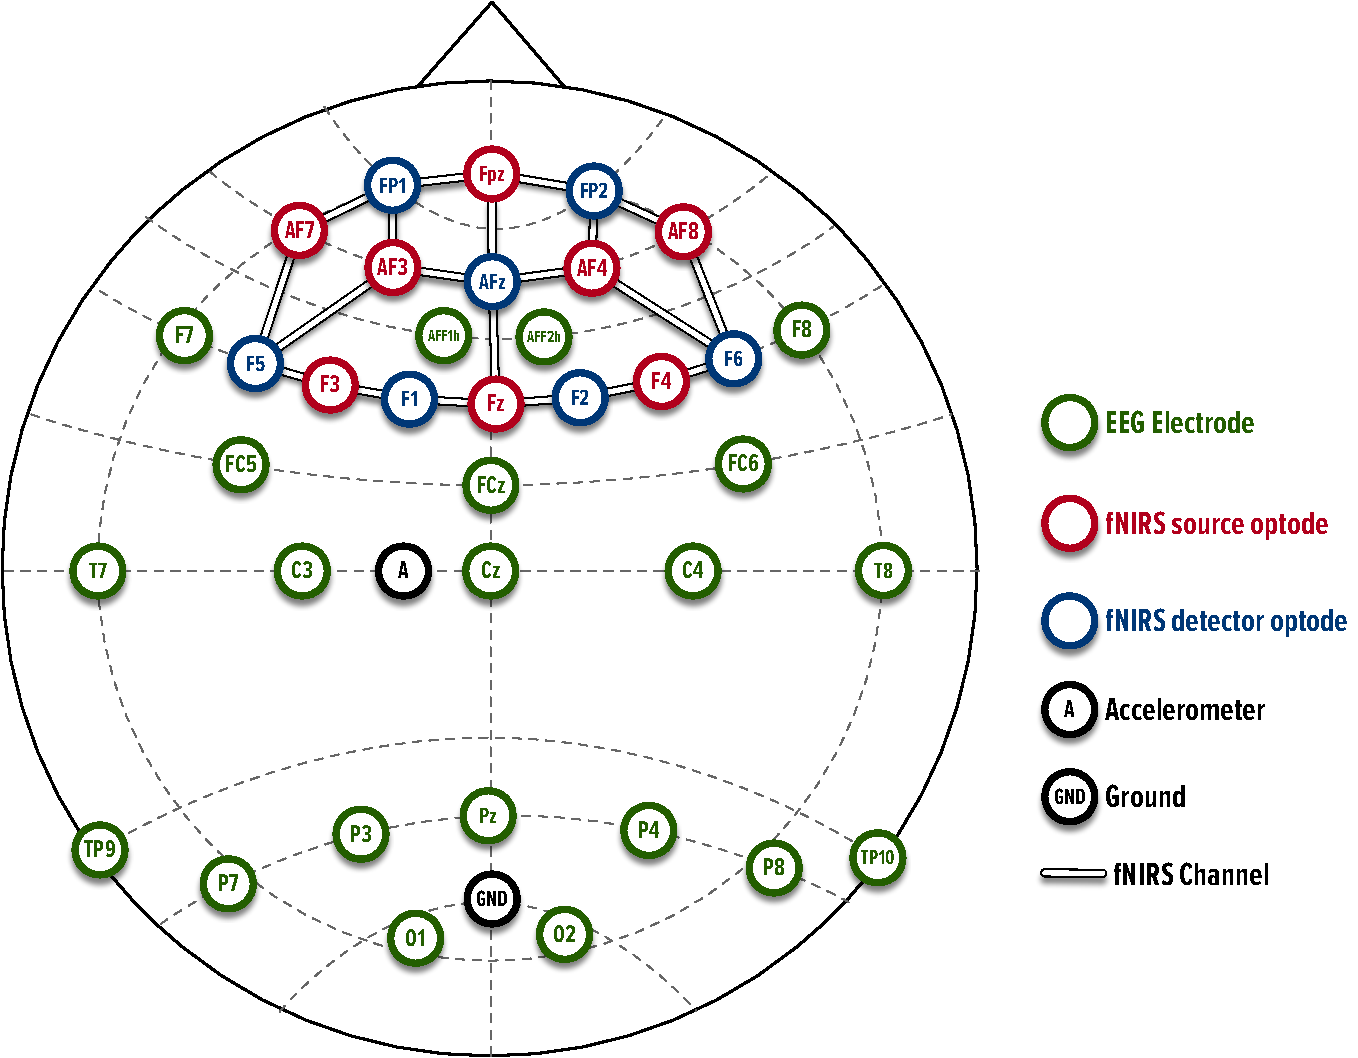
\includegraphics[width=\linewidth]{images/combined_montage.pdf}
  \centering
  \caption{%
      The montage we used for combined EEG/fNIRS data acquisition.  EEG
      electrodes were located in the anterior frontal (AFF1h, AFF2h), frontal
      (F7, F8), frontocentral (FC5, FCz, FC6), central (C3, Cz, C4),
      occipital (O1, O2), temporal (T7, T8) and parietal (P7, P3, Pz, P4, P8)
      regions.  fNIRS optodes were located in frontal (Fz, F1, F2, F3, F4,
      F5, F6), anterior frontal (AF3, AF4, AFz, AF7, AF8), frontal polar
      (FP1, FPz, FP2). The line is the channel formed when fNIRS source
      optode (red) and fNIRS detector (blue) optode are combined.
  }
  \label{fig:combined-montage}
\end{figure}

\begin{table}
\centering
\begin{tabularx}{\textwidth}{lX}
    \toprule
    EEG signal columns & Description (topological location of the subject's brain) \\
    \midrule
    \texttt{<subject>\_eeg\_AFF1h} & Left anterior frontal region \\
    \texttt{<subject>\_eeg\_F7} & Left frontal region  \\
    \texttt{<subject>\_eeg\_FC5} & Left fronto-central region  \\
    \texttt{<subject>\_eeg\_C3} & Left central region \\
    \texttt{<subject>\_eeg\_T7} & Left temporal region \\
    \texttt{<subject>\_eeg\_TP9} & Left temporal-parietal region \\
    \texttt{<subject>\_eeg\_Pz} & Central parietal region \\
    \texttt{<subject>\_eeg\_P3} & Left parietal region \\
    \texttt{<subject>\_eeg\_P7} & Left parietal region \\
    \texttt{<subject>\_eeg\_O1} & Left occipital region \\
    \texttt{<subject>\_eeg\_O2} & Right occipital region \\
    \texttt{<subject>\_eeg\_P8} & Right parietal region \\
    \texttt{<subject>\_eeg\_P4} & Right parietal region \\
    \texttt{<subject>\_eeg\_TP10} & Right temporal-parietal region \\
    \texttt{<subject>\_eeg\_Cz} & central region \\
    \texttt{<subject>\_eeg\_C4} & Right central region \\
    \texttt{<subject>\_eeg\_T8} & Right temporal region \\
    \texttt{<subject>\_eeg\_FC6} & Right fronto-central region \\
    \texttt{<subject>\_eeg\_FCz} & Central fronto-central region \\
    \texttt{<subject>\_eeg\_F8} & Right frontal region \\
    \texttt{<subject>\_eeg\_AFF2h} & Right anterior frontal region \\
    \texttt{<subject>\_eeg\_GSR} & Right hand \\
    \texttt{<subject>\_eeg\_EKG} & 4\textsuperscript{th} Intercostal space \\
    \bottomrule
\end{tabularx}
\caption{EEG signal descriptions, specifying the topological locations on the subject's brain. Each entry provides the label of the signal column corresponding to the EEG electrode location. For a visual representation of these electrode locations, refer to \autoref{fig:combined-montage}.
}
\label{tab:EEG_signals}
\end{table}

\begin{table}
  \centering
  \begin{tabularx}{\textwidth}{lX}
  \toprule
  fNIRS raw signal columns & Description (topological location of the subject's brain) \\
  \midrule
  \texttt{<subject>\_fnirs\_S1-D1\_760} & 'F3-F5': left frontal region \\
  \texttt{<subject>\_fnirs\_S1-D2\_760} & 'F3-F1': left frontal region  \\
  \texttt{<subject>\_fnirs\_S2-D1\_760} & 'Af7-F5': left anterior frontal region  \\
  \texttt{<subject>\_fnirs\_S2-D3\_760} & 'Af7-Fp1': left anterior frontal region  \\
  \texttt{<subject>\_fnirs\_S3-D1\_760} & 'Af3-F5': left anterior frontal region  \\
  \texttt{<subject>\_fnirs\_S3-D3\_760} & 'Af3-Fp1': left anterior frontal region  \\
  \texttt{<subject>\_fnirs\_S3-D4\_760} & 'Af3-Afz': left anterior frontal region  \\
  \texttt{<subject>\_fnirs\_S4-D2\_760} & 'Fz-F1': left frontal region  \\
  \texttt{<subject>\_fnirs\_S4-D4\_760} & 'Fz-Afz': central frontal region  \\
  \texttt{<subject>\_fnirs\_S4-D5\_760} & 'Fz-F2': right frontal region  \\
  \texttt{<subject>\_fnirs\_S5-D3\_760} & 'Fpz-Fp1': left frontal polar region  \\
  \texttt{<subject>\_fnirs\_S5-D4\_760} & 'Fpz-Afz': central frontal polar region  \\
  \texttt{<subject>\_fnirs\_S5-D6\_760} & 'Fpz-Fp2': right frontal polar region  \\
  \texttt{<subject>\_fnirs\_S6-D4\_760} & 'Af4-Afz': right anterior frontal region  \\
  \texttt{<subject>\_fnirs\_S6-D6\_760} & 'Af4-Fp2': right anterior frontal region  \\
  \texttt{<subject>\_fnirs\_S6-D7\_760} & 'Af4-F6': right anterior frontal region  \\
  \texttt{<subject>\_fnirs\_S7-D5\_760} & 'F4-F2': right frontal region  \\
  \texttt{<subject>\_fnirs\_S7-D7\_760} & 'F4-F6': right frontal region  \\
  \texttt{<subject>\_fnirs\_S8-D6\_760} & 'Af8-Fp2': right anterior frontal region  \\
  \texttt{<subject>\_fnirs\_S8-D7\_760} & 'Af8-F6': right anterior frontal region  \\
  \texttt{<subject>\_fnirs\_S1-D1\_850} & 'F3-F5': left frontal region  \\
  \texttt{<subject>\_fnirs\_S1-D2\_850} & 'F3-F1': left frontal region  \\
  \texttt{<subject>\_fnirs\_S2-D1\_850} & 'Af7-F5': left anterior frontal region  \\
  \texttt{<subject>\_fnirs\_S2-D3\_850} & 'Af7-Fp1': left anterior frontal region  \\
  \texttt{<subject>\_fnirs\_S3-D1\_850} & 'Af3-F5': left anterior frontal region  \\
  \texttt{<subject>\_fnirs\_S3-D3\_850} & 'Af3-Fp1': left anterior frontal region  \\
  \texttt{<subject>\_fnirs\_S3-D4\_850} & 'Af3-Afz': left anterior frontal region  \\
  \texttt{<subject>\_fnirs\_S4-D2\_850} & 'Fz-F1': left frontal region  \\
  \texttt{<subject>\_fnirs\_S4-D4\_850} & 'Fz-Afz': central frontal region  \\
  \texttt{<subject>\_fnirs\_S4-D5\_850} & 'Fz-F2': right frontal region  \\
  \texttt{<subject>\_fnirs\_S5-D3\_850} & 'Fpz-Fp1': left frontal polar region  \\
  \texttt{<subject>\_fnirs\_S5-D4\_850} & 'Fpz-Afz': central frontal polar region  \\
  \texttt{<subject>\_fnirs\_S5-D6\_850} & 'Fpz-Fp2': right frontal polar region  \\
  \texttt{<subject>\_fnirs\_S6-D4\_850} & 'Af4-Afz': right anterior frontal region  \\
  \texttt{<subject>\_fnirs\_S6-D6\_850} & 'Af4-Fp2': right anterior frontal region  \\
  \texttt{<subject>\_fnirs\_S6-D7\_850} & 'Af4-F6': right anterior frontal region  \\
  \texttt{<subject>\_fnirs\_S7-D5\_850} & 'F4-F2': right frontal region  \\
  \texttt{<subject>\_fnirs\_S7-D7\_850} & 'F4-F6': right frontal region  \\
  \texttt{<subject>\_fnirs\_S8-D6\_850} & 'Af8-Fp2': right anterior frontal region  \\
  \texttt{<subject>\_fnirs\_S8-D7\_850} & 'Af8-F6': right anterior frontal region  \\
  \bottomrule
  \end{tabularx}
  \caption{Table of fNIRS raw signal descriptions, mapping the source (S) to the detector (D) for various topological locations on the subject's brain. These signals where recorded using the Aurora fNIRS software. Each channel is recorded using light wavelengths of 760nm and 850nm. For a visual representation of these electrode locations, refer to \autoref{fig:combined-montage}.}
  \label{tab:fNIRS_raw_signals}
  \end{table}

  \begin{table}
    \centering
    \begin{tabularx}{\textwidth}{lX}
    \toprule
    fNIRS raw signal columns & Description (topological location of the subject's brain) \\
    \midrule
    \texttt{<subject>\_fnirs\_S1-D1\_HbO} & 'F3-F5': left frontal region \\
    \texttt{<subject>\_fnirs\_S1-D2\_HbO} & 'F3-F1': left frontal region  \\
    \texttt{<subject>\_fnirs\_S2-D1\_HbO} & 'Af7-F5': left anterior frontal region  \\
    \texttt{<subject>\_fnirs\_S2-D3\_HbO} & 'Af7-Fp1': left anterior frontal region  \\
    \texttt{<subject>\_fnirs\_S3-D1\_HbO} & 'Af3-F5': left anterior frontal region  \\
    \texttt{<subject>\_fnirs\_S3-D3\_HbO} & 'Af3-Fp1': left anterior frontal region  \\
    \texttt{<subject>\_fnirs\_S3-D4\_HbO} & 'Af3-Afz': left anterior frontal region  \\
    \texttt{<subject>\_fnirs\_S4-D2\_HbO} & 'Fz-F1': left frontal region  \\
    \texttt{<subject>\_fnirs\_S4-D4\_HbO} & 'Fz-Afz': central frontal region  \\
    \texttt{<subject>\_fnirs\_S4-D5\_HbO} & 'Fz-F2': right frontal region  \\
    \texttt{<subject>\_fnirs\_S5-D3\_HbO} & 'Fpz-Fp1': left frontal polar region  \\
    \texttt{<subject>\_fnirs\_S5-D4\_HbO} & 'Fpz-Afz': central frontal polar region  \\
    \texttt{<subject>\_fnirs\_S5-D6\_HbO} & 'Fpz-Fp2': right frontal polar region  \\
    \texttt{<subject>\_fnirs\_S6-D4\_HbO} & 'Af4-Afz': right anterior frontal region  \\
    \texttt{<subject>\_fnirs\_S6-D6\_HbO} & 'Af4-Fp2': right anterior frontal region  \\
    \texttt{<subject>\_fnirs\_S6-D7\_HbO} & 'Af4-F6': right anterior frontal region  \\
    \texttt{<subject>\_fnirs\_S7-D5\_HbO} & 'F4-F2': right frontal region  \\
    \texttt{<subject>\_fnirs\_S7-D7\_HbO} & 'F4-F6': right frontal region  \\
    \texttt{<subject>\_fnirs\_S8-D6\_HbO} & 'Af8-Fp2': right anterior frontal region  \\
    \texttt{<subject>\_fnirs\_S8-D7\_HbO} & 'Af8-F6': right anterior frontal region  \\
    \texttt{<subject>\_fnirs\_S1-D1\_HbR} & 'F3-F5': left frontal region  \\
    \texttt{<subject>\_fnirs\_S1-D2\_HbR} & 'F3-F1': left frontal region  \\
    \texttt{<subject>\_fnirs\_S2-D1\_HbR} & 'Af7-F5': left anterior frontal region  \\
    \texttt{<subject>\_fnirs\_S2-D3\_HbR} & 'Af7-Fp1': left anterior frontal region  \\
    \texttt{<subject>\_fnirs\_S3-D1\_HbR} & 'Af3-F5': left anterior frontal region  \\
    \texttt{<subject>\_fnirs\_S3-D3\_HbR} & 'Af3-Fp1': left anterior frontal region  \\
    \texttt{<subject>\_fnirs\_S3-D4\_HbR} & 'Af3-Afz': left anterior frontal region  \\
    \texttt{<subject>\_fnirs\_S4-D2\_HbR} & 'Fz-F1': left frontal region  \\
    \texttt{<subject>\_fnirs\_S4-D4\_HbR} & 'Fz-Afz': central frontal region  \\
    \texttt{<subject>\_fnirs\_S4-D5\_HbR} & 'Fz-F2': right frontal region  \\
    \texttt{<subject>\_fnirs\_S5-D3\_HbR} & 'Fpz-Fp1': left frontal polar region  \\
    \texttt{<subject>\_fnirs\_S5-D4\_HbR} & 'Fpz-Afz': central frontal polar region  \\
    \texttt{<subject>\_fnirs\_S5-D6\_HbR} & 'Fpz-Fp2': right frontal polar region  \\
    \texttt{<subject>\_fnirs\_S6-D4\_HbR} & 'Af4-Afz': right anterior frontal region  \\
    \texttt{<subject>\_fnirs\_S6-D6\_HbR} & 'Af4-Fp2': right anterior frontal region  \\
    \texttt{<subject>\_fnirs\_S6-D7\_HbR} & 'Af4-F6': right anterior frontal region  \\
    \texttt{<subject>\_fnirs\_S7-D5\_HbR} & 'F4-F2': right frontal region  \\
    \texttt{<subject>\_fnirs\_S7-D7\_HbR} & 'F4-F6': right frontal region  \\
    \texttt{<subject>\_fnirs\_S8-D6\_HbR} & 'Af8-Fp2': right anterior frontal region  \\
    \texttt{<subject>\_fnirs\_S8-D7\_HbR} & 'Af8-F6': right anterior frontal region  \\
    \bottomrule
    \end{tabularx}
    \caption{%
        fNIRS raw signal descriptions, mapping the source (S) to the detector
        (D) for various topological locations on the subject's brain. HbO, or
        oxyhemoglobin, and HbR, or deoxyhemoglobin, are the two types of
        hemoglobin measured. For a visual representation of these electrode
        locations, refer to \autoref{fig:combined-montage}.
    }
    \label{tab:fNIRS_signals}
    \end{table}

\section{Derived data}

\subsection{Synchronization of EEG, EKG, GSR, and fNIRS Signals}

In multimodal neuroimaging studies, synchronizing signals from multiple modalities is a crucial step to conducting comprehensive studies on all these modalities together. The discrepancy between EEG and fNIRS signals' time series is an issue that researchers encounter frequently due to the limitations of recording hardware or the necessity to remove invalid signals. Additionally, these two modalities have distinct recording rates, further complicating their alignment. To facilitate comprehensive evaluation of EEG and fNIRS signals, it is essential to synchronize these two signals.

We plotted histograms of the EEG and fNIRS signals to check they were sampled at the expected hardware frequency (10Hz for fNIRS and 500Hz for EEG). This is important because the filtering step assumes samples are equally spaced. Having confirmed that, the synchronization process is a two-step approach involving the noise artifacts removal from the signals, followed by resampling and synchronization of the interpolated signals at the desired sampling rate.

\subsubsection{Removing Noise in EEG Signals with Notch Filter}

EEG signals often exhibit susceptibility to artifacts, an interference that can be attributed to several sources. For instance, physiological factors such as eye movements or blinks can induce such artifacts \cite{10.3389/fnhum.2012.00278}, as can environmental elements like fluorescent lighting or grounding complications \cite{Kaya21}.

Upon thorough examination and visualization of the raw EEG data, we identified a consistent 60 Hz electrical disturbance within the signal, along with corresponding harmonics. An anomalous peak was also noted around the 5 Hz mark, potentially attributable to a grounding irregularity or an other environmental factors.

With the aid of MNE-Python \cite{GramfortEtAl2013a}, we efficiently mitigated these intrusive noises by deploying a notch filter. The filter was configured with a frequency of 60 Hz, a transition bandwidth of 9 Hz, and notch widths of 2 Hz.

\subsubsection{Mitigating Artifacts in fNIRS Signals Utilizing Bandpass Filter}

fNIRS signals are often susceptible to motion artifacts (MA) stemming from physiological activities, including cardiac and respiratory disturbances. These artifacts become particularly noticeable in the measurement of oxyhemoglobin (HbO) and deoxyhemoglobin (HbR) concentrations within the signal channels.

To address these challenges, we employed a bandpass filter as an effective noise reduction strategy. The filter was calibrated in line with the recommendations provided by \cite{Koenraadt2014}. With a low cutoff bandwidth of 0.01 Hz and a high cutoff bandwidth of 0.2 Hz for the 4th order Butterworth method, the filter was tailored to selectively allow signal components within this frequency range while attenuating components outside the range.

\subsubsection{Pre-processing EKG and GSR Signals}

To remove noise and improve peak-detection accuracy for EKG signals, we employed a finite impulse response (FIR) filter with 0.67 Hz low cutoff frequency, 45 Hz high cutoff frequency, and order of $1.5 \times \text{sampling rate}$ (where sampling rate is 500 Hz) implemented by NeuroKit2 \cite{Makowski2021neurokit}.

We removed noise and smoothed the GSR signals using a low-pass filter with a 3 Hz cutoff frequency and a $4^\text{th}$ order Butterworth filter, both implemented by Neurokit2.

\subsubsection{Synchronization of EEG, EKG, GSR, and fNIRS Signals}

After the EEG, EKG, GSR, and fNIRS signals are pre-processed to remove noise, the signals are upsampled to 2000Hz using the FFT-based resampling method \texttt{mne.filter.resample} available in the Python MNE library \cite{GramfortEtAl2013a}. 

For each experiment, we define a common clock with initial time starting 2 minutes before the beginning of the first task (rest state) and end time set to 2 minutes after the final task (typically Minecraft). We create equally spaced ticks in this clock at the frequency of 200Hz. Then, the signals are downsampled to this clock's scale via linear interpolation. 

\subsubsection{Mapping to the Task Data}

Mapping between signals and data will depend on the task being performed. For instance, one can choose to map a signal to the closest data observation or a collection of them. Therefore, we opted for providing the timestamp as a column in the synchronized signals tables so that they can be used for alignment with the task observations.

\newpage
\bibliographystyle{ieeetr}
\bibliography{references}

\end{document}
